 \documentclass[rgb]{beamer}
\usepackage{silence,lmodern}
\usepackage[backend=biber, style=ieee]{biblatex}
\usepackage{csquotes}
\usepackage{listings}
\usepackage{svg}
\usepackage{multirow}
\usepackage{booktabs}
\usepackage{multicol}
\usepackage{forest}
\usepackage[format=plain, justification=justified, labelfont=bf, textfont=it, font=small, labelsep=space]{caption}
\usepackage{appendixnumberbeamer}

\WarningFilter{biblatex}{Patching footnotes failed}
\WarningFilter{etex}{Extended allocation already in use}

\renewcommand*{\bibfont}{\tiny}
\bibliography{resources.bib}

\usetheme{Konstanz}
\setcounter{secnumdepth}{3}
\format{169}


\title{Locality Optimization for traversal-based Queries on Graph Databases}
\titleCorporateDesign{Locality Optimization}{for traversal-based}{Queries on}{Graph Databases}
\author{Fabian Klopfer} 
\date{30.04.2021}
\institute{Databases and Information Systems Group \\ Department of Computer and Information Science \\ University of Konstanz}

\AtBeginDocument{
\usebeamerfont{normalfont}
\begin{frame}
	\titlepage
\end{frame}
}

\begin{document}
\section{Introduction}
        
        \begin{frame}{Graphs}
            \begin{figure}
                \begin{center}
                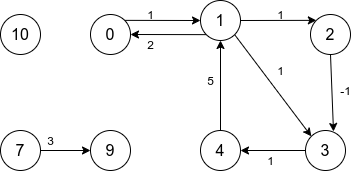
\includegraphics[keepaspectratio, height=0.8\textheight, width=0.6\textwidth]{img/data_struct_gr.png}
                \end{center}
            \end{figure}
        \end{frame}

         \begin{frame}[allowframebreaks]{Data Structures}
            Two essential record structures: \\ [2em]
            \begin{enumerate}
                \item Node records \\ [2em]
                \item Relationship records \\ [3em]
            \end{enumerate}
            Inspired by Neo4J~\autocite{robinson2015graph, Rodriguez2010ConstructionsFD}.
            
            \framebreak
            \begin{figure}
                \begin{center}
                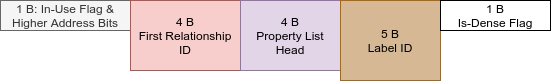
\includegraphics[keepaspectratio, height=\textheight, width=\textwidth]{img/node_record.png}
                \end{center}
            \end{figure}
            
            \framebreak
            \begin{figure}
                \begin{center}
                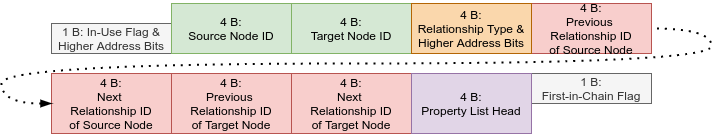
\includegraphics[keepaspectratio, height=\textheight, width=\textwidth]{img/relationship_record.png}
                \end{center}
            \end{figure}
        \end{frame}
        
        \begin{frame}[fragile]{Data Structures -- Example}
            \begin{figure}
                \begin{center}
                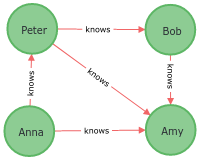
\includegraphics[keepaspectratio, height=0.4\textheight, width=.4\textwidth]{img/graph.png}
                \end{center}
            \end{figure}
            \end{frame}
            
            \begin{frame}
            \begin{figure}
                \begin{center}
                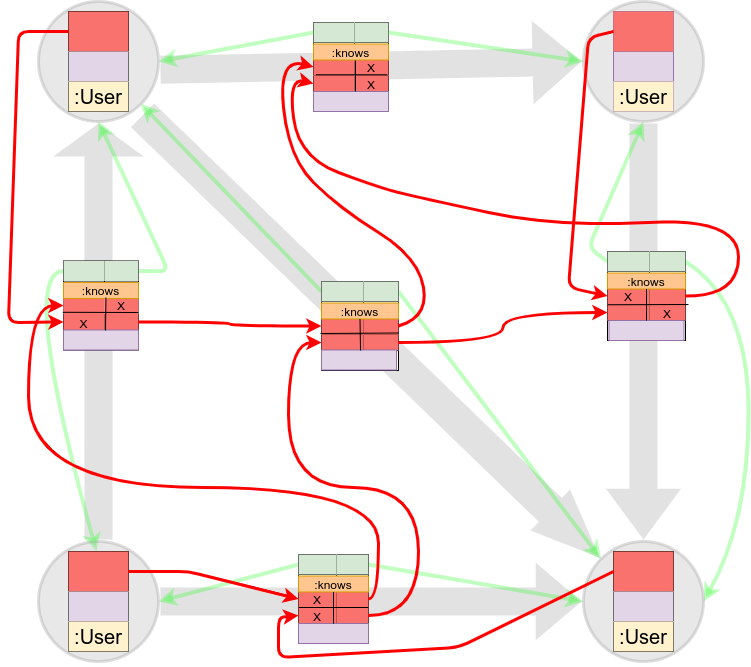
\includegraphics[keepaspectratio, height=\textheight, width=\textwidth]{img/example_structs.png}
                \end{center}
            \end{figure}
        \end{frame}
    
    \begin{frame}[fragile]{Example Query}        
        Show me all people that Bob knows:
        
        \begin{figure}[htp]
            \begin{center}
            \begin{forest}
                [ $\uparrow_x^y$
                    [ $\sigma_{x.\text{name = 'Bob'}}$ ($\bigcirc$ x) ]
                ]
                \end{forest} 
            \end{center}        
        \end{figure}
        
        $\Rightarrow$ Scaning and filtering read sequential. \\ [1em]
        $\Rightarrow$ \texttt{Expand} does not necessarily. \\ [1em]
    \end{frame}
    
    \begin{frame}{Traversal-based Query}
        \begin{figure}
            \begin{center}
            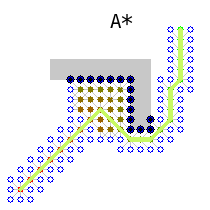
\includegraphics[keepaspectratio, height=0.6\textheight, width=0.6\textwidth]{img/astar.png}
            \end{center}
        \end{figure}
    \end{frame}

    
     \begin{frame}{Motivation}    
        \begin{itemize}
            \item \texttt{Expand}'s access pattern depends on the query, record and incidence list order. \\ [2em]
            \item When these factors are not considered, access is random. \\ [1em]
            Potentially leads to \\ [0.5em]
               \begin{itemize}
                    \item[$\Rightarrow$] hard-to-predict access patterns.
                    \item[$\Rightarrow$] cache \& prefetch misses, thrashing and pollution.
                    \item[$\Rightarrow$] inadequate page eviction behavior. \\ [2em]
                \end{itemize}
        \end{itemize}
        \alert{Traversals rely primarily on \texttt{expand}!}
    \end{frame}
    
\section{Problem Definition}
    \begin{frame}[allowframebreaks]{Locality}
            \begin{itemize}
                \item  ``memory references tend to be localized in time and space''~\autocite{jacob2010memory}. \\ [2em]
                \item Tendency to access nearby memory locations based on previous accesses~\autocite{denning2006locality}. \\ [2em]
                \item Enables usage of memory hierarchy. \\ [3em]
            \end{itemize}
            
            $\Rightarrow$ The more localized the access the less IO ops are necessary~\autocite{gupta2013locality}.

         \framebreak
            Temporal locality based on blocks 
                \[ P (X_{t + \Delta} = B | X_t = B) \] \\ [2em]
            Spatial locality in the same sense 
                \[ P(X_{t + \Delta} = B \pm \varepsilon | X_t = B) \] 
                with $\varepsilon = \lceil \frac{p}{b} \rceil$~\autocite{gupta2013locality}.
          
        \end{frame}

     \begin{frame}{Problem Definition}
            Given a graph $G$, logical block size $b$, page size $p$. \\ [2em]
            Desired is \\ [1em]
            \begin{enumerate}
            \item A partition of $G$ into blocks of size $b$, \\ [1em]
            \item permutations $\pi_v, \pi_e$ of the blocks,\\ [1.5em]
            \end{enumerate}
            such that locality is as high as possible for traversal-based queries.
    \end{frame}
    
    \begin{frame}[fragile]{Example: Block Formation and Order}
            \begin{figure}[htp]
                \begin{center}
                    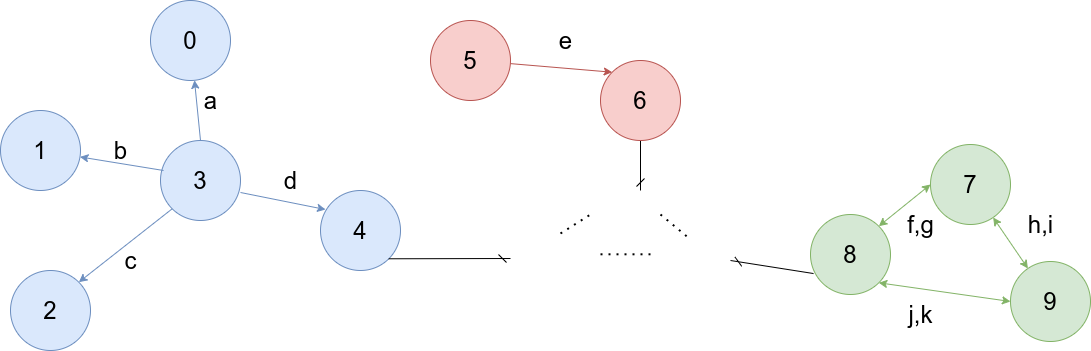
\includegraphics[keepaspectratio,height=0.4\textheight,width=\textwidth]{img/example_graph.png}
                \end{center}
            \end{figure}
            
             \begin{table}[htp]
                \centering
                \begin{tabular}[c]{|l|c|c|c|c|c|c|} \hline
                &&&&&&\\[-1em]
                node.db & \colorbox{blue!30}{0}, \colorbox{red!30}{5}, \colorbox{green!30}{7} & \colorbox{blue!30}{1}, \colorbox{blue!30}{4}, \colorbox{green!30}{9} & \colorbox{blue!30}{2}, \colorbox{red!30}{6}, \colorbox{green!30}{8} & \colorbox{blue!30}{3} &  & \\ \hline
                &&&&&&\\[-1em]
                edge.db & \colorbox{blue!30}{a}, \colorbox{green!30}{f} & \colorbox{blue!30}{b}, \colorbox{green!30}{g} & \colorbox{blue!30}{c}, \colorbox{green!30}{h} & \colorbox{blue!30}{d}, \colorbox{green!30}{i} & \colorbox{red!30}{e}, \colorbox{green!30}{j} & \colorbox{green!30}{k} \\  \hline
                \end{tabular}
                \vspace{0.5cm}
                
                \begin{tabular}{|l | c | c | c | c | c | c|} \hline
                &&&&&&\\[-1em]
                node.db & \colorbox{green!30}{7},\colorbox{green!30}{8}, \colorbox{green!30}{9} & \colorbox{blue!30}{0}, \colorbox{blue!30}{1}, \colorbox{blue!30}{3} & \colorbox{blue!30}{2}, \colorbox{blue!30}{4}, \colorbox{red!30}{5} & \colorbox{red!30}{6} &  & \\ \hline
                &&&&&&\\[-1em]
                 edge.db &  \colorbox{green!30}{f}, \colorbox{green!30}{h} & \colorbox{green!30}{g}, \colorbox{green!30}{k} & \colorbox{green!30}{i}, \colorbox{green!30}{j} & \colorbox{blue!30}{a}, \colorbox{blue!30}{b} & \colorbox{blue!30}{c}, \colorbox{blue!30}{d} & \colorbox{red!30}{e} \\ \hline
                \end{tabular}
            \end{table}
        \end{frame}       
        
\section{Locality-optimizing Record Layout}
    \begin{frame}{Record Layout Methods: Overview}
        \begin{itemize}
            \item Existing methods \\ [0.5em]
            \begin{itemize}
                \item G-Store~\autocite{steinhaus2010g} \\ [0.5em]
                \item ICBL~\autocite{yacsar2017distributed} \\ [2em]
            \end{itemize}
            
            \item Our approach \\ [0.5em]
            \begin{itemize}
             \item Community detection --- Louvain method~\autocite{blondel2008fast}. \\ [0.5em]
             \item Incidence list reordering
            \end{itemize}
        \end{itemize}
    \end{frame}

        \begin{frame}[allowframebreaks, fragile]{G-Store}
            \begin{figure}[H]
                \begin{center}
                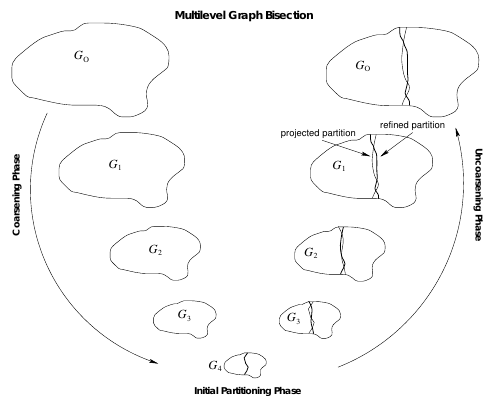
\includegraphics[keepaspectratio, height=0.8\textheight, width=\textwidth]{img/multilevel.png}\\
                \end{center}
            \end{figure}
            
            \framebreak
            \vfill\vspace{0pt}
            \begin{enumerate}
             \item Coarsening: Heavy-Edge Matching~\autocite{karypis}
             \item Turn-around
             \item Uncoarsening
                \begin{enumerate}
                 \item Project
                 \item Reorder
                 \item Refine\\ [3em]
                \end{enumerate}
            \end{enumerate}
             \[ \min \sum_{(u,v) \in E} |\phi(u) - \phi(v)| \] 
             
            \framebreak
            \begin{figure}[H]
                \begin{center}
                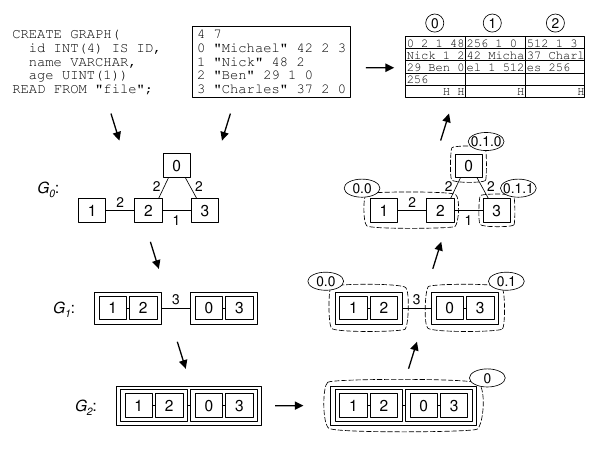
\includegraphics[keepaspectratio, height=0.9\textheight, width=\textwidth]{img/g-store.png}\\
                \end{center}
            \end{figure}
            \vfill\vspace{0pt}
        \end{frame}
        
        \begin{frame}[allowframebreaks]{ICBL}
        \vspace{-3.3em}
            \begin{figure}
                \begin{center}
                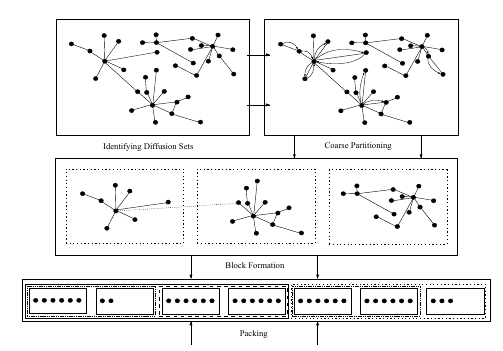
\includegraphics[keepaspectratio, height=\textheight, width=\textwidth]{img/icbl.png}
                \end{center}
            \end{figure}
            
            \framebreak
            \begin{enumerate}
             \item[I ] Feature extraction: Do $t$ random walks~\autocite{fouss2007random} of length $l$. 
             \item[C] Coarse clustering: Adapted K-Means~\autocite{lloyd1982least}.
             \item[B] Block Formation: Agglomerative hierarchical clustering~\autocite{hac}.
             \item[L] Layout Blocks: Sort blocks and subgraphs
            \end{enumerate}

            
        \end{frame}
        
        \begin{frame}[allowframebreaks]{Louvain Method}
            \begin{figure}
                \begin{center}
                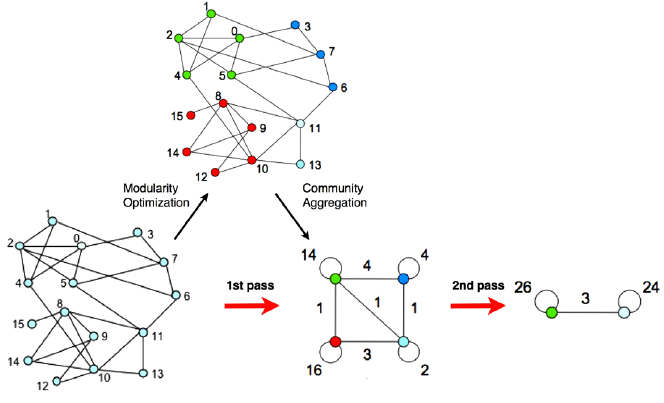
\includegraphics[keepaspectratio, height=0.8\textheight, width=.8\textwidth]{img/louvain.png}
                \end{center}
            \end{figure}
            
            \framebreak
            
            \begin{enumerate}
             \item Initialize all nodes in singleton community.
             \item Merge community into a neighboring community where modularity gain is maximal, until modularity gain is below threshold.
             \item Construct new graph from aggregated communities and go to 1.
            \end{enumerate}
            \vspace{2em}
            \[ \frac{1}{2m} \sum_{u,v \in V} \left( w_{(u, v)} - \frac{w_u w_v}{2m} \right) \cdot \delta (c_u, c_v) \]
            
        \end{frame}
        
        \begin{frame}{Incidence List Rearrangement}
            \begin{figure}
                \begin{center}
                    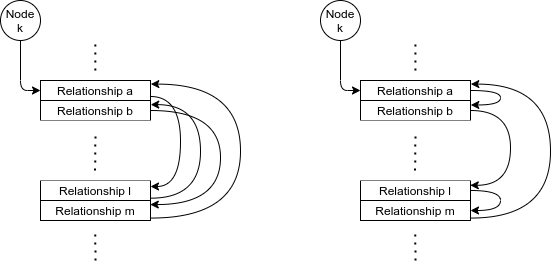
\includegraphics[keepaspectratio, height=0.65\textheight, width=.65\textwidth]{img/incl.png}
                \end{center}
            \end{figure}
        \end{frame}
        
    \section{Evaluation}
        \begin{frame}[allowframebreaks]{Setup}
            \begin{itemize}
            \item Queries: BFS, DFS, Dijkstra, A$^*$, ALT. \\ [3em]       
                \begin{figure}
                    \begin{center}
                    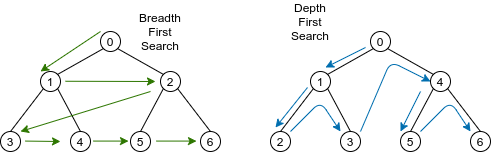
\includegraphics[keepaspectratio, height=0.4\textheight, width=0.75\textwidth]{img/bfs-dfs.png} \hspace{0.7cm}
                    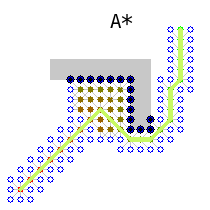
\includegraphics[keepaspectratio, height=0.4\textheight, width=0.2\textwidth]{img/astar.png}
                    \end{center}
                \end{figure}
                
                \framebreak
            \item Datasets: $[131, 1'134'890]$ nodes, $[764, 2'987'624]$ edges, average degree $[2.6, 25.5]$ \\ [3em]
            \item Domains include biological neural net, e-mails, co-authors, frequent item sets, video channel subscriptions~\autocite{snap}.
            \end{itemize}
        \framebreak
        
            \begin{itemize}
            \item Simulate IOs using in-memory access layer, queries and record IDs. \\ [1em]
            \item Block no. $=$ record ID $\cdot$ \texttt{sizeof(}record struct\texttt{)} $/$ block size \\  [1em]
            \item Consecuive accesses to same block require no IO op. \\ [1em]
            \item All other accesses count as one IO op. \\ [2em]
            \end{itemize}
            \begin{enumerate}
                \item Import dataset.
                \item Run query and log IDs of accessed nodes and relationships.
                \item Calculate sequence of block no. from sequence of IDs.
                \item Calculate sequence of page no. from sequence of block no.
               \end{enumerate}
        \end{frame}
        
        \begin{frame}[allowframebreaks]{Results}
            \begin{figure}
                \begin{center}
                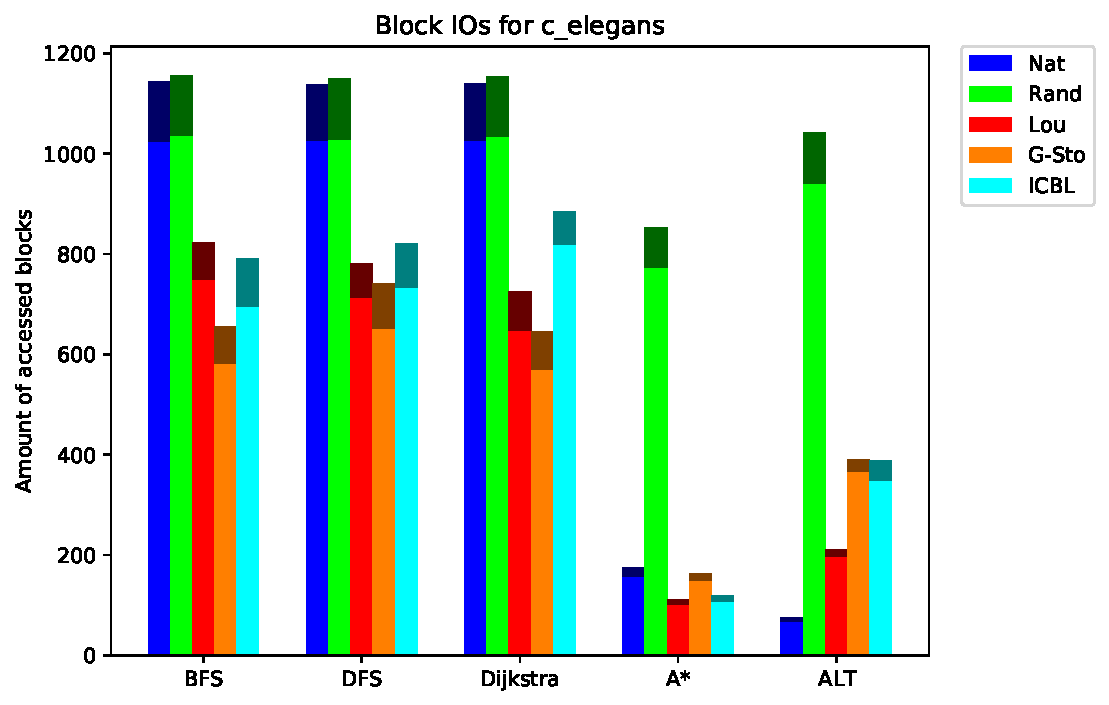
\includegraphics[keepaspectratio, height=\textheight, width=.45\textwidth]{img/c_elegans_Block_unsorted_io_comparison.pdf} \hfill
                 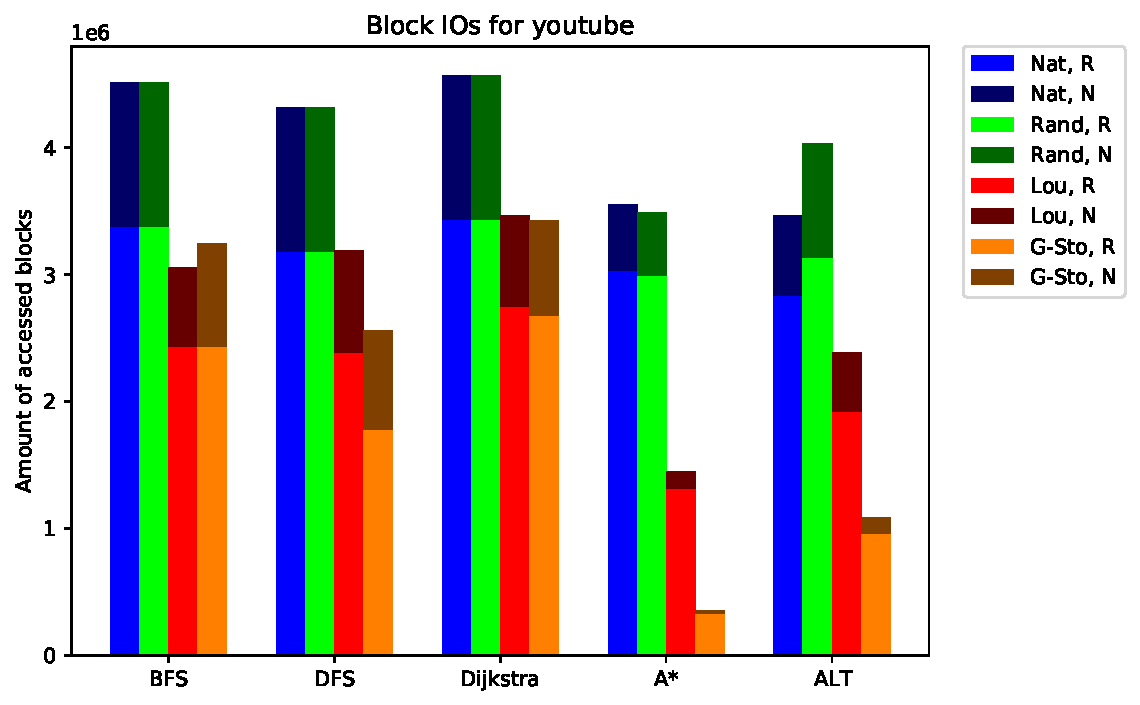
\includegraphics[keepaspectratio, height=\textheight, width=.45\textwidth]{img/youtube_Block_unsorted_io_comparison.pdf}
                \end{center}
            \end{figure}
            
            \framebreak
            \begin{figure}
                \begin{center}
                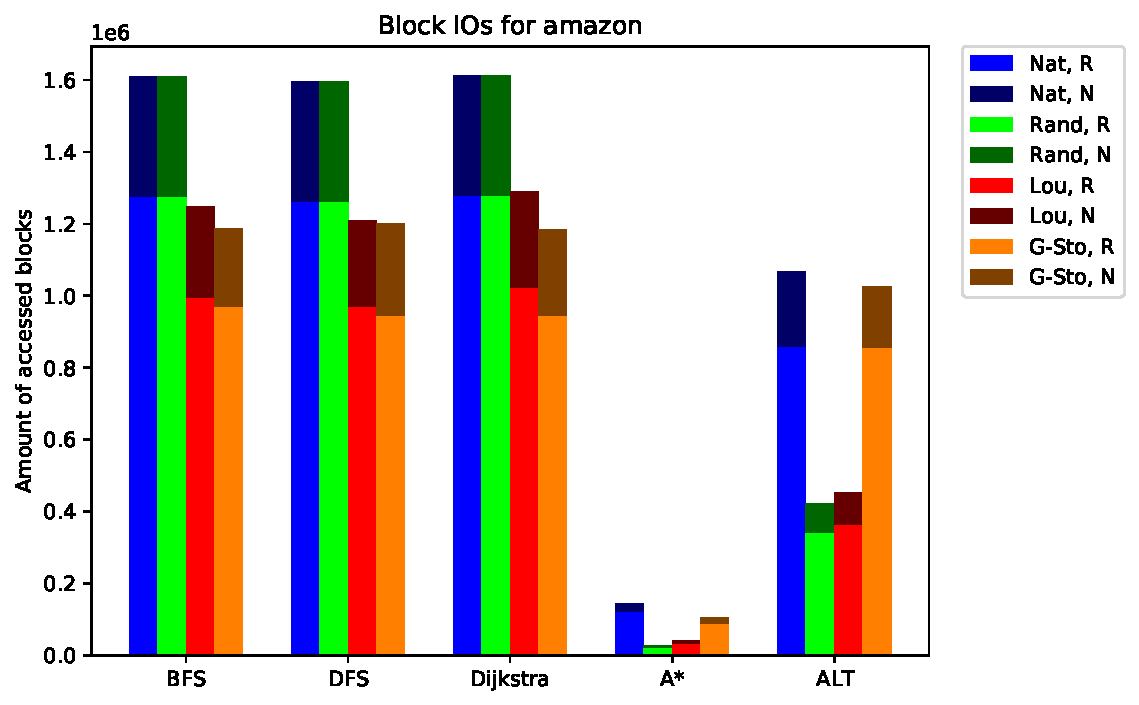
\includegraphics[keepaspectratio, height=0.8\textheight, width=0.45\textwidth]{img/amazon_Block_unsorted_io_comparison.pdf} \hfill
                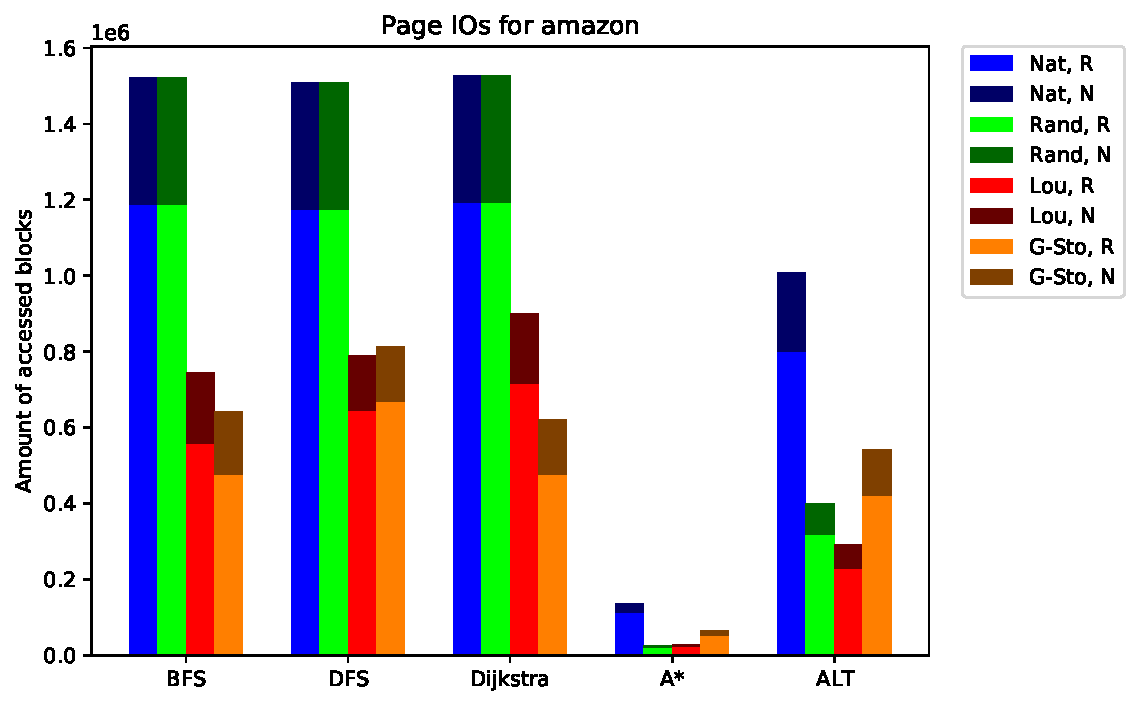
\includegraphics[keepaspectratio, height=0.8\textheight, width=0.45\textwidth]{img/amazon_Page_unsorted_io_comparison.pdf}
                \end{center}
            \end{figure}

            \framebreak
            \begin{figure}
                \begin{center}
                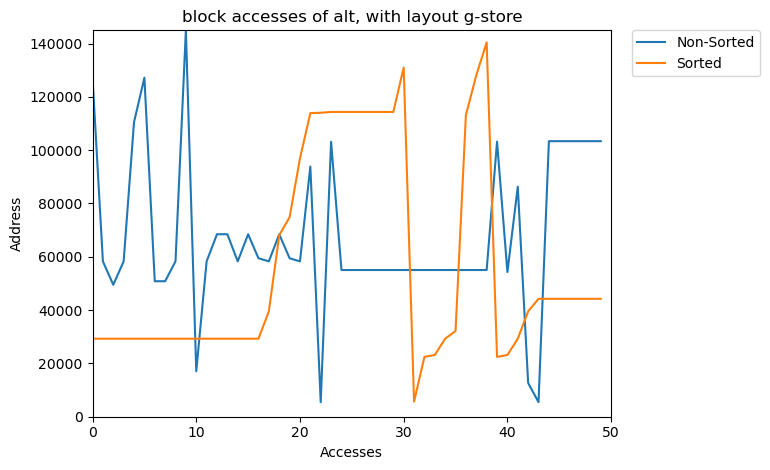
\includegraphics[keepaspectratio, height=0.8\textheight, width=.45\textwidth]{img/dblp_g-store_alt_block_sil_access_seq.png} \hfill
                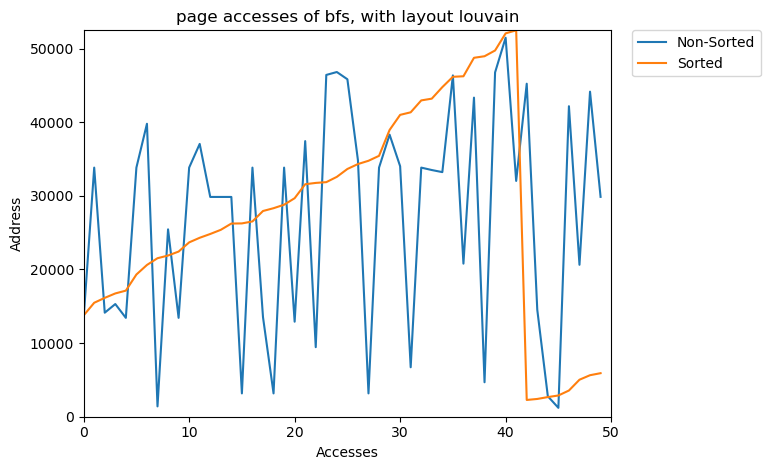
\includegraphics[keepaspectratio, height=0.8\textheight, width=.45\textwidth]{img/youtube_louvain_bfs_page_sil_access_seq.png}
                \end{center}
            \end{figure}
            
            \framebreak
            \begin{figure}
                \begin{center}
                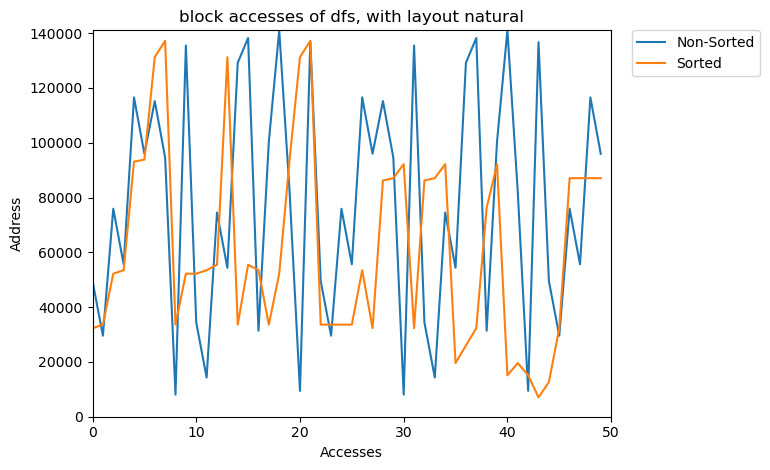
\includegraphics[keepaspectratio, height=0.8\textheight, width=\textwidth]{img/dblp_natural_dfs_block_sil_access_seq.png}
                \end{center}
            \end{figure}
        \end{frame}
    
    \section{Conclusion}
        \begin{frame}{Summary}
            \begin{itemize}
                \item Static rearrangement methods increase locality. \\ [0.5em]
                $\Rightarrow$ decrease number of block accesses \\ [3em]
                \item The order of blocks is important for spatial locality \\ [3em]
                \item Sorting the incidence lists leads to more sequential access sequences. \\ [3em]
                \item Results differ between queries 
                \end{itemize}
        \end{frame}
    
        \begin{frame}{Future Work}
        \begin{itemize}
            \item Leiden~\autocite{traag2019louvain} instead of Louvain \\ [2em]
            \item RCM-based~\autocite{Cuthill1969ReducingTB} rearrangement \\ [2em]
            \item  Dynamic Rearrangement \\ [1.5em]
                \begin{itemize}
                 \item Query-based \\ [1em]
                 \item History-based 
                \end{itemize}

        \end{itemize}
        \end{frame}
        
\section{References}
    \begin{frame}[allowframebreaks]
    \nocite{*}
      \begin{tiny}
      \printbibliography
      \end{tiny}
    \end{frame}
\end{document}
